\documentclass[a4paper,14pt]{extarticle}

\usepackage[utf8x]{inputenc}
\usepackage[T1,T2A]{fontenc}
\usepackage[russian]{babel}
\usepackage{hyperref}
\usepackage{indentfirst}
\usepackage{here}
\usepackage{array}
\usepackage{graphicx}
\usepackage{caption}
\usepackage{subcaption}
\usepackage{chngcntr}
\usepackage{amsmath}
\usepackage{amssymb}
\usepackage{pgfplots}
\usepackage{pgfplotstable}
\usepackage[left=2cm,right=2cm,top=2cm,bottom=2cm,bindingoffset=0cm]{geometry}
\usepackage{multicol}
\usepackage{askmaps}
\usepackage{titlesec}
\usepackage{listings}
\usepackage{color}
\usepackage{courier}

\definecolor{green}{rgb}{0,0.6,0}
\definecolor{gray}{rgb}{0.5,0.5,0.5}
\definecolor{purple}{rgb}{0.58,0,0.82}

\lstset{
	language=Verilog,
	backgroundcolor=\color{white},   
	basicstyle=\small\ttfamily,
	commentstyle=\color{green},
	keywordstyle=\color{blue},	
	numberstyle=\tiny\color{gray},
	stringstyle=\color{purple},
	breakatwhitespace=false,
	breaklines=true,
	captionpos=b,
	keepspaces=true,
	numbers=left,
	numbersep=5pt,
	showspaces=false,
	showstringspaces=false,
	showtabs=false,
	tabsize=4,
	frame=single,
	inputpath={../quartus/},
	literate={~} {$\sim$}{1}
}

\renewcommand{\le}{\ensuremath{\leqslant}}
\renewcommand{\leq}{\ensuremath{\leqslant}}
\renewcommand{\ge}{\ensuremath{\geqslant}}
\renewcommand{\geq}{\ensuremath{\geqslant}}
\renewcommand{\epsilon}{\ensuremath{\varepsilon}}
\renewcommand{\phi}{\ensuremath{\varphi}}
\renewcommand{\thefigure}{\arabic{figure}} 	
\renewcommand*\not[1]{\overline{#1}}

\titleformat*{\section}{\large\bfseries} 
\titleformat*{\subsection}{\normalsize\bfseries} 
\titleformat*{\subsubsection}{\normalsize\bfseries} 
\titleformat*{\paragraph}{\normalsize\bfseries} 
\titleformat*{\subparagraph}{\normalsize\bfseries} 

\counterwithin{figure}{section}
\counterwithin{equation}{section}
\counterwithin{table}{section}
\newcommand{\sign}[1][5cm]{\makebox[#1]{\hrulefill}}
\graphicspath{{../pics/}}
\captionsetup{justification=centering,margin=1cm}
\def\arraystretch{1.3}
\setlength\parindent{5ex}
\titlelabel{\thetitle.\quad}

\begin{document}

\begin{titlepage}
\begin{center}
	Санкт-Петербургский Политехнический Университет Петра Великого\\[0.3cm]
	Институт компьютерных наук и технологий \\[0.3cm]
	Кафедра компьютерных систем и программных технологий\\[4cm]
	
	\textbf{ОТЧЕТ}\\ 
	\textbf{по лабораторной работе}\\[0.5cm]
	\textbf{SystemVerilog №4}\\[0.1cm]
	Автоматизация проектирования\\ дискретных устройств\\[4.0cm]
\end{center}

\begin{flushright}
	\begin{minipage}{0.45\textwidth}
		\textbf{Работу выполнил студент}\\[3mm]
		группа 33501/4 \hspace*{9mm} Дьячков В.В.\\[5mm]
		\textbf{Преподаватель}\\[5mm]
		\sign[1.5cm] \hspace*{1mm} к.т.н., доц. Филиппов А.С. \\[5mm]
	\end{minipage}
\end{flushright}

\vfill

\begin{center}
	Санкт-Петербург\\
	\the\year
\end{center}
\end{titlepage}

\addtocounter{page}{1}
\counterwithin{lstlisting}{section}

\tableofcontents
\newpage
\listoffigures
\lstlistoflistings
\newpage

\section{lab7\_1}

\subsection{Задание}

На языке Verilog создайте описание:
\begin{itemize}
	\item Task (задачи) сортировки двух чисел (комбинационная схема):
		\begin{itemize}
			\item Передаваемые значений: два числа \code{a} и \code{b};
			\item Возвращаемые значения: \code{min} – меньшее из \code{a} и \code{b}; \code{max} – большее из \code{a} и \code{b}.
		\end{itemize}
	\item Устройства (комбинационная схема) сортировки четырех 2-разрядных чисел, использующего созданную задачу.
	\item Параметр \code{INV} -- инверсия выходных данных устройства ($=1$ выходные данные инвертируются; $=0$ выходные данные не инвертируются).
	\item Входы:
		\begin{itemize}
			\item Переключатель \code{sw[7:6]} -- операнд A;
			\item Переключатель \code{sw[5:4]} -- операнд B;
			\item Переключатель \code{sw[3:2]} -- операнд C;
			\item Переключатель \code{sw[1:0]} -- операнд D.
		\end{itemize}
	\item Выходы: операнды, отсортированные по убыванию:
		\begin{itemize}
			\item Светодиоды \code{led[7:6]};
			\item Светодиоды \code{led[5:4]};
			\item Светодиоды \code{led[3:2]};
			\item Светодиоды \code{led[1:0]}.
		\end{itemize}
\end{itemize}

Дополнительные требования:
\begin{itemize}
	\item[$\circ$] Стандарты и номера выводов СБИС для платы miniDiLaB\_CIV задать с помощью атрибутов.
	\item[$\circ$] Осуществите функциональное моделирование при \code{INV = 0}.
	\item[$\circ$] Проверку на плате осуществите при \code{INV = 1}.
\end{itemize}
В описании можно использовать любые операторы.

\subsection{Код на языке Verilog}

В листинге \ref{code:1} приведен код программы на языке Verilog.

\lstinputlisting[caption=lab7\_1.v, label=code:1]{lab7_1/lab7_1.v}

\newpage

\subsection{Результаты синтеза}

На рис. \ref{fig:lab7_1_rtl} приведено изображение синтезированной схемы в RLT Viewer.
\begin{figure}[H]
\begin{center}
	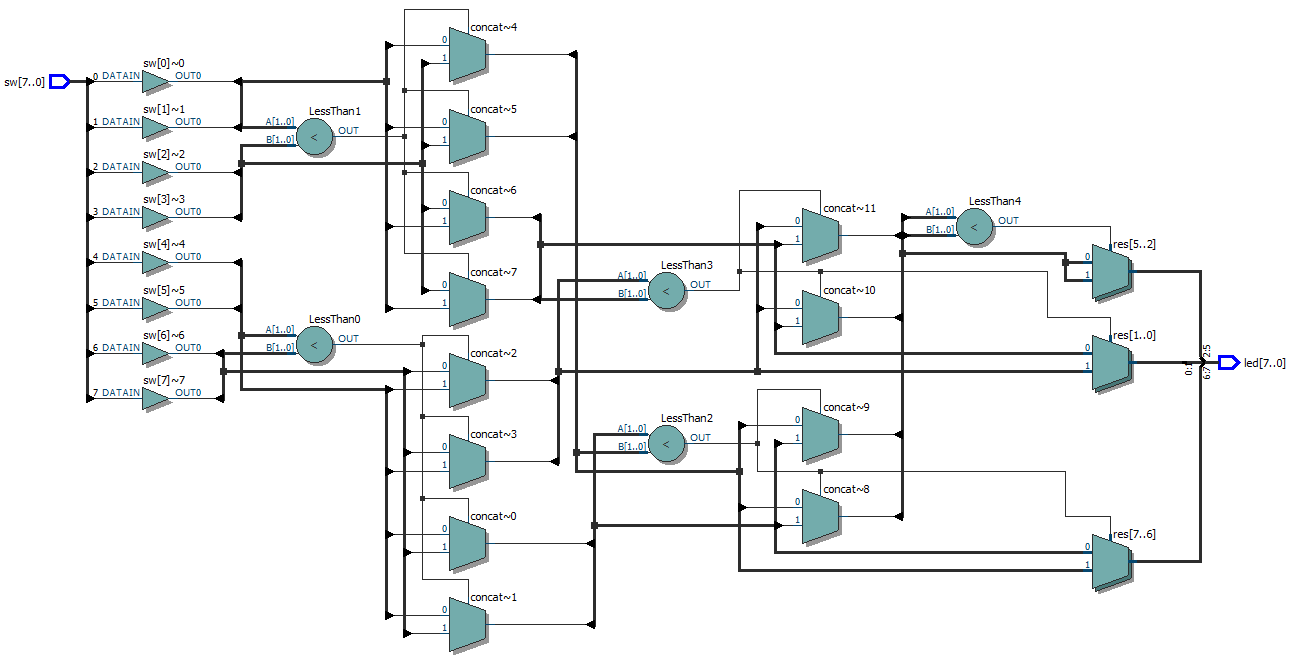
\includegraphics[width=\textwidth]{lab7_1_rtl}
	\caption{Результат синтеза в RLT Viewer}
	\label{fig:lab7_1_rtl}
\end{center}
\end{figure}
\vspace{-1cm}

\subsection{Результаты моделирования}
\label{sec:lab7_1_modeling}

На рис. \ref{fig:lab7_1_modeling} изображена временная диаграмма работы синтезированного устройства при \code{INV = 0}. На вход подаются четыре случайных значения, которые сортируются и записываются в порядке убывания значения.

\begin{figure}[H]
\begin{center}
	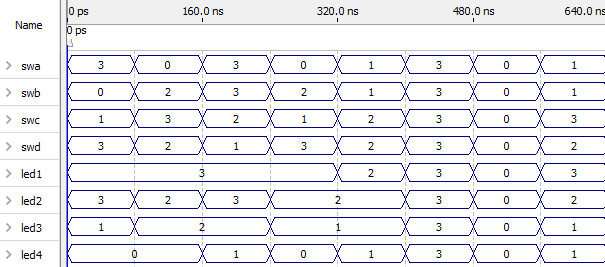
\includegraphics[width=\textwidth]{lab7_1_modeling}
	\caption{Результаты моделирования}
	\label{fig:lab7_1_modeling}
\end{center}
\end{figure}

\subsection{Назначение выводов СБИС}

На рис. \ref{fig:lab7_1_pins} приведены назначения выводов СБИС в Pin Planner.

\begin{figure}[H]
\begin{center}
	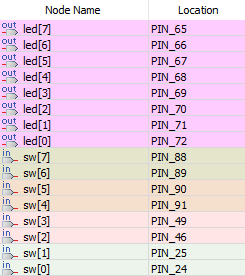
\includegraphics{lab7_1_pins}
	\caption{Таблица назначений в Pin Planer}
	\label{fig:lab7_1_pins}
\end{center}
\end{figure}

\subsection{Результаты проверки на плате}

Для тестирования проекта на плате были использованы тесты, описанные в пункте \ref{sec:lab7_1_modeling} при \code{INV = 1}. Результаты тестирования совпадают с ожидаемыми, следовательно, устройство работает верно.

\subsection{Выводы}

Реализовано параметризированное устройства сортировки четырех 2-разрядных чисел на основе описанной задачи сортировки двух чисел. Результаты моделирования и тестирования на плате показали, что разработанное устройство работает верно.

\newpage

\section{lab7\_2}

\subsection{Задание}

В пакете QII введите приведенное ниже Verilog описание кольцевого сдвигающего регистра, имеющего:
\begin{itemize}
	\item Входы данных \code{da}, \code{db}, \code{dc};
	\item Вход выбора источника загрузки данных в регистр -- \code{sel};
	\item Вход синхронной загрузки данных в регистр -- \code{load}.
\end{itemize}

\lstinputlisting[caption=latch\_ff\_n.v, label=code:2]{lab7_2/latch_ff_n.v}

\begin{itemize}
	\item Запустите полную компиляцию модуля.
	\item Найдите сообщения о триггерах-защелках (привести в отчете).
	\item Найдите триггеры-защелки в RTL Viewer (привести в отчете).
	\item Зафиксируйте аппаратные затраты на реализацию модуля -- число логических элементов (привести в отчете).
	\item Исправьте описание так, чтобы не порождался ни один триггер-защелка
	\item Запустите полную компиляцию модуля.
	\item Убедитесь, что нет сообщений о триггерах-защелках.
	\item Убедитесь, что нет триггеров-защелок в RTL Viewer (привести в отчете).
	\item Зафиксируйте аппаратные затраты на реализацию модуля -- число логических элементов (привести в отчете).
	\item Осуществите моделирование при \code{N = 4}.
\end{itemize}

\subsection{Результаты компиляции}

В результате компиляции исходного проекта были получены следующие предупреждения о триггерах-защелках:
\begin{itemize}
	\item \textbf{Warning (13004)}: Presettable and clearable registers converted to equivalent circuits with latches. Registers power-up to an undefined state, and DEVCLRn places the registers in an undefined state.
	\item \textbf{Warning (13012)}: Latch temp[0] has unsafe behavior.
	\item \textbf{Warning (13012)}: Latch temp[1] has unsafe behavior.
	\item \textbf{Warning (13012)}: Latch temp[2] has unsafe behavior.
	\item \textbf{Warning (13012)}: Latch temp[3] has unsafe behavior.
	\item \textbf{Warning (335093)}: TimeQuest Timing Analyzer is analyzing 8 combinational loops as latches.
\end{itemize}

На рис. \ref{fig:lab7_2_rtl_1} приведено изображение синтезированной схемы в RLT Viewer. Красным цветом на схеме отмечены триггеры-защелки. Аппаратурные затраты составили 20 ЛЭ, включая 2 регистра.
\begin{figure}[H]
\begin{center}
	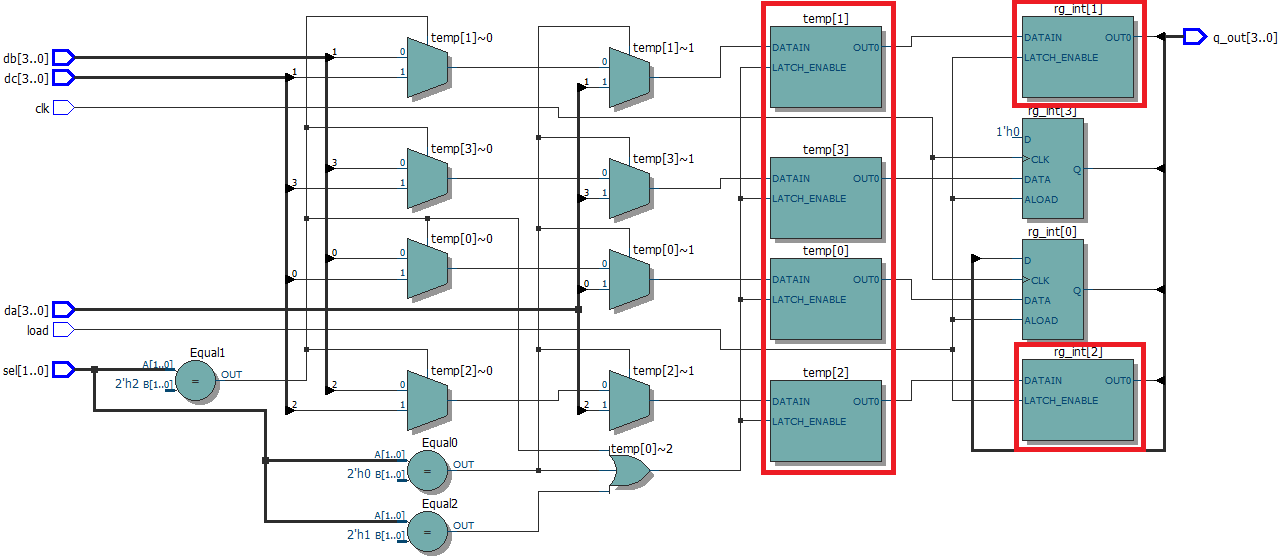
\includegraphics[width=0.95\textwidth]{lab7_2_rtl_1}
	\caption{Результат синтеза в RLT Viewer}
	\label{fig:lab7_2_rtl_1}
\end{center}
\end{figure}

\subsection{Исправленное описание на языке Verilog}

В листинге \ref{code:2} приведен код программы на языке Verilog, не порождающий ни одного триггера-защелки.

\lstinputlisting[caption=lab7\_2.v, label=code:2]{lab7_2/lab7_2.v}

\newpage

\subsection{Результаты синтеза}

На рис. \ref{fig:lab7_2_rtl} приведено изображение синтезированной схемы в RLT Viewer. Видно, что триггеров-защелок не появилось. Аппаратурные затраты составили 20 ЛЭ, включая 4 регистра.

\begin{figure}[H]
\begin{center}
	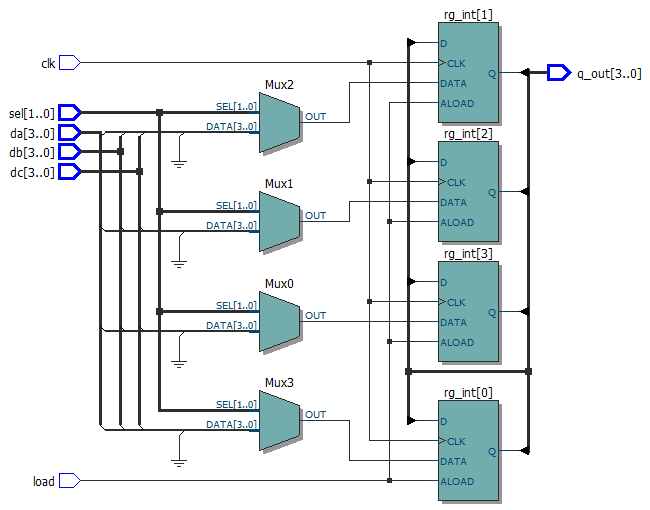
\includegraphics[width=0.9\textwidth]{lab7_2_rtl_2}
	\caption{Результат синтеза в RLT Viewer}
	\label{fig:lab7_2_rtl}
\end{center}
\end{figure}

\newpage

\subsection{Результаты моделирования}
\label{sec:lab7_2_modeling}

На рис. \ref{fig:lab7_2_modeling} изображена временная диаграмма работы синтезированного устройства при \code{N = 4}.

\begin{figure}[H]
\begin{center}
	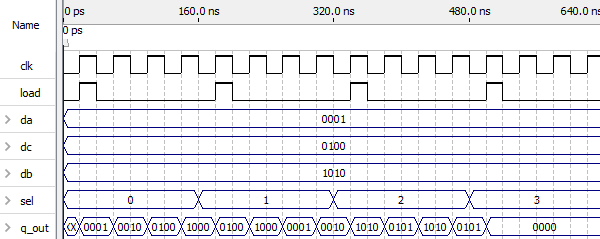
\includegraphics[width=\textwidth]{lab7_2_modeling}
	\caption{Результаты моделирования}
	\label{fig:lab7_2_modeling}
\end{center}
\end{figure}

\subsection{Выводы}

Реализовано описание кольцевого сдвигающего регистра, не порождающего триггеров-защелок. Результаты моделирования показали, что разработанное устройство работает верно.

\newpage

\section{elab7\_1}

\subsection{Задание}

На языке Verilog создайте структурное описание параметризированного устройства (параметр \code{INV = 1} -- инверсия выходных данных), приведенного на рис. \ref{fig:elab7_1_0}.

\begin{figure}[H]
\begin{center}
	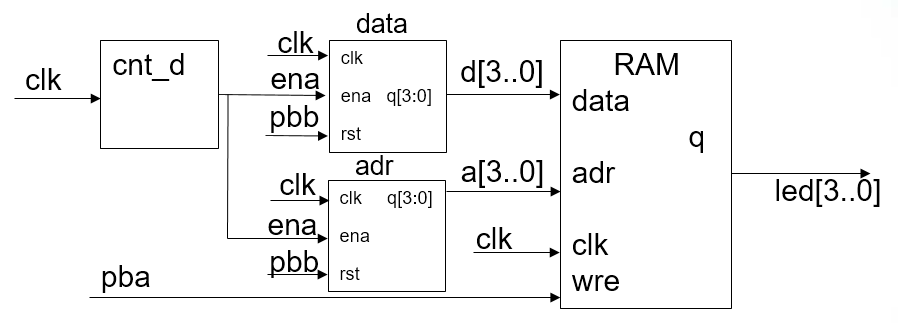
\includegraphics[width=\textwidth]{elab7_1_0}
	\caption{Параметризированное устройство}
	\label{fig:elab7_1_0}
\end{center}
\end{figure}
\vspace{-0.5cm}

В состав устройства входят:
\begin{itemize}
	\item \code{cnt_d} -- cчетчик делитель (параметр -- \code{DIV}), обеспечивающий счет по модулю \code{DIV} (базовое значение -- $3$) и формирование синхронного сигнала переноса (активный уровень сигнала -- $1$, длительность один такт тактовой частоты) по достижению счетчиком значения \code{DIV - 1}.
	\item \code{data} -- формирователь данных для модуля памяти (реализован на базе параметризированного счетчика \code{cnt_N}).
	\item \code{adr} -- формирователь адреса для модуля памяти (реализован на базе параметризированного счетчика \code{cnt_N}).
	\item \code{RAM} -- модуль памяти (параметры: \code{word_num} -- число слов (базовое значение $16$), \code{data_W} -- разрядность данных (базовое значение $4$); простая одно портовая память с чтением новых данных в процессе записи):
		\begin{itemize}
			\item Для расчета разрядности шины адреса следует использовать функцию с постоянным значением для вычисления $\log_2($\code{word_num}$)$;
			\item Вход \code{wre} – вход разрешения записи ($=1$ -- запись в память разрешена);
			\item Модуль памяти должен быть инициализирован данными: \code{4'h0} -- четные адреса; \code{4'hf} -- нечетные адреса.
		\end{itemize}
	\item \code{cnt_N} -- двоичный счетчик на сложение с параметризированной разрядностью (параметр \code{N}, базовое значение -- $4$), имеющий вход тактовых сигналов (\code{clk}), вход разрешения работы (\code{ena}), вход асинхронного сброса (\code{rst}) и выход -- \code{q[N-1:0]}.
	\item Входы:
		\begin{itemize}
			\item Кнопка \code{pbb} -- вход асинхронного сброса (кнопка нажата – сброс);
			\item Кнопка \code{pba} -- вход разрешения записи в память (кнопка нажата – запись разрешена);
			\item Тактовый сигнал (\code{clk}) подается от тактового генератора. Частота тактового сигнала -- 25МГц.
		\end{itemize}
	\item Выходы: светодиоды \code{led[3:0]} -- выходы устройства.
\end{itemize}

Дополнительные требования:
\begin{itemize}
	\item[$\circ$] Стандарты и номера выводов СБИС для платы miniDiLaB\_CIV задать с помощью атрибутов.
	\item[$\circ$] Осуществите функциональное моделированиеми  модулей \code{cnt_d}, \code{cnt_N}, \code{RAM} с базовыми значениями параметров.
	\item[$\circ$] Осуществите функциональное моделирование устройства при: \code{DIV = 3}, \code{N = 4}, \code{word_num = 16}, \code{data_W = 4}, \code{INV = 0}.
	\item[$\circ$] Проверку устройства на плате осуществите при: \code{DIV = 25_000_000}, \code{N = 4}, \code{word_num = 16}, \code{data_W = 4}, \code{INV = 1}.
\end{itemize}
В описании можно использовать любые операторы.

\newpage

\subsection{Код на языке Verilog}

В листинге \ref{code:5} приведен код программы на языке Verilog.

\lstinputlisting[caption=elab7\_1.v, label=code:5]{elab7_1/elab7_1.v}

\newpage

\lstinputlisting[caption=cnt\_d.v, label=code:6]{elab7_1/cnt_d.v}

\lstinputlisting[caption=cnt\_N.v, label=code:6]{elab7_1/cnt_N.v}

\newpage

\lstinputlisting[caption=RAM.v, label=code:6]{elab7_1/RAM.v}

\newpage

\subsection{Результаты синтеза}

На рис. \ref{fig:elab7_1_rtl} -- \ref{fig:elab7_1_rtl_3} приведены изображения синтезированного устройства и каждого модуля по отдельности в RLT Viewer.

\begin{figure}[H]
\begin{center}
	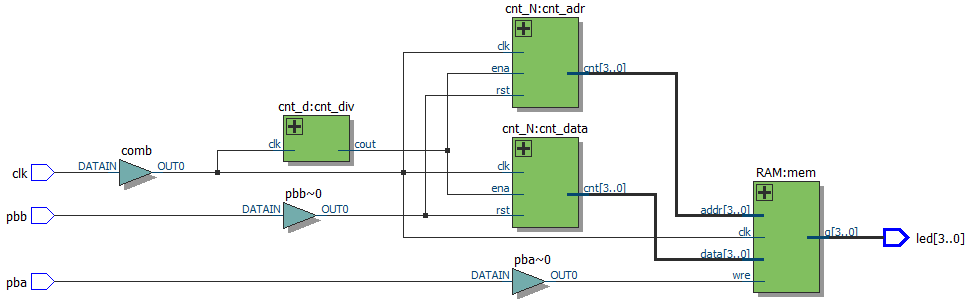
\includegraphics[width=\textwidth]{elab7_1_rtl}
	\caption{Результат синтеза устройства в RLT Viewer}
	\label{fig:elab7_1_rtl}
\end{center}
\end{figure}

\begin{figure}[H]
\begin{center}
	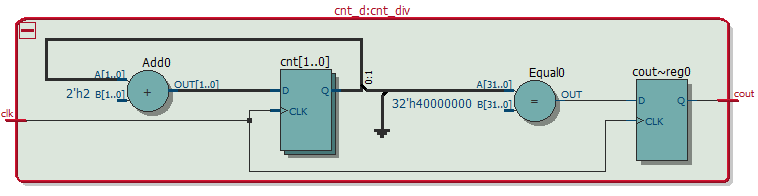
\includegraphics[width=\textwidth]{elab7_1_rtl_1}
	\caption{Результат синтеза \code{cnt_div} в RLT Viewer}
	\label{fig:elab7_1_rtl_1}
\end{center}
\end{figure}

\begin{figure}[H]
\begin{center}
	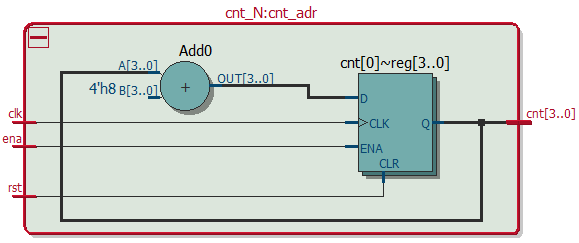
\includegraphics[width=0.7\textwidth]{elab7_1_rtl_2}
	\caption{Результат синтеза \code{cnt_adr} в RLT Viewer}
	\label{fig:elab7_1_rtl_2}
\end{center}
\end{figure}

\begin{figure}[H]
\begin{center}
	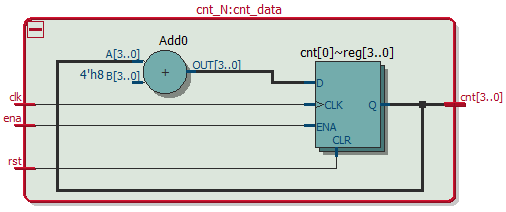
\includegraphics[width=0.7\textwidth]{elab7_1_rtl_3}
	\caption{Результат синтеза \code{cnt_data} в RLT Viewer}
	\label{fig:elab7_1_rtl_3}
\end{center}
\end{figure}

\subsection{Результаты моделирования}
\label{sec:elab7_1_modeling}

На рис. \ref{fig:elab7_1_modeling_1} -- \ref{fig:elab7_1_modeling} изображены временные диаграммы работы каждого модуля по отдельности и всего синтезированного устройства при \code{DIV = 3},\\ \code{N = 4}, \code{word_num = 16}, \code{data_W = 4}, \code{INV = 0}.

\begin{figure}[H]
\begin{center}
	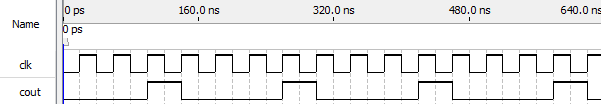
\includegraphics[width=\textwidth]{elab7_1_modeling_1}
	\caption{Результаты моделирования модуля \code{cnt_d}}
	\label{fig:elab7_1_modeling_1}
\end{center}
\end{figure}

\begin{figure}[H]
\begin{center}
	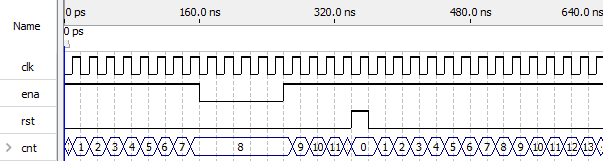
\includegraphics[width=\textwidth]{elab7_1_modeling_2}
	\caption{Результаты моделирования модуля \code{cnt_N}}
	\label{fig:elab7_1_modeling_2}
\end{center}
\end{figure}

\begin{figure}[H]
\begin{center}
	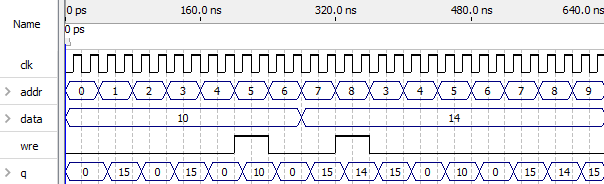
\includegraphics[width=\textwidth]{elab7_1_modeling_3}
	\caption{Результаты моделирования модуля \code{RAM}}
	\label{fig:elab7_1_modeling_3}
\end{center}
\end{figure}

\begin{figure}[H]
\begin{center}
	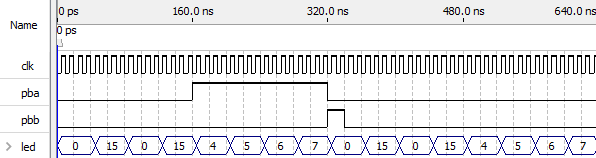
\includegraphics[width=\textwidth]{elab7_1_modeling}
	\caption{Результаты моделирования устройства}
	\label{fig:elab7_1_modeling}
\end{center}
\end{figure}

При моделировании устройства при активном уровне \code{pba} происходит запись в память, а при активном уровне \code{pbb} происходит асинхронный сброс. Сначала происходит чтение начальных данных, затем запись в память, после чего происходит асинхронный сброс и чтение записанных ранее данных.

\subsection{Назначение выводов СБИС}

На рис. \ref{fig:elab7_1_pins} приведены назначения выводов СБИС в Pin Planner.

\begin{figure}[H]
\begin{center}
	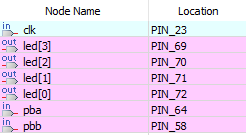
\includegraphics{elab7_1_pins}
	\caption{Таблица назначений в Pin Planer}
	\label{fig:elab7_1_pins}
\end{center}
\end{figure}

\subsection{Результаты проверки на плате}

Для тестирования проекта на плате были использованы тесты, описанные в пункте \ref{sec:elab7_1_modeling} при параметрах \code{DIV = 25_000_000}, \code{N = 4}, \code{word_num = 16}, \code{data_W = 4}, \code{INV = 1}. Результаты тестирования совпадают с ожидаемыми, следовательно, устройство работает верно.

\subsection{Выводы}

Реализовано описание параметризированного устройства, включающего счетчик-делитель, формирователи данных и адреса, модуль памяти и двоичный счетчик на сложение. Результаты моделирования и тестирования на плате показали, что разработанное устройство работает верно.

\end{document}